\chapter{Project description}
\textit{This chapter seeks to explain the design and implementation of the project along with the tests used for improving the system.}
\section{Architecture}
The architecture of the system explains the conceptual design blocks and interfaces. The system consist of the CDU and a number of sensor nodes as seen on figure \ref{fig:systembdd}. The CDU is responsible for contacting the sensor nodes in order to collect and store the data that has been acquired by the sensor nodes. The sensor nodes sole responsibility is to acquire data.\\
The supply for the sensors nodes is taken from the custom power line communication bus. Communication signals between the CDU and sensor nodes are found on the bus as well.\\ 
\begin{figure}[H]
	\centering
	\includegraphics[width=.9\textwidth]{billeder/11ProjectDescription/systembdd}
	\caption{System overview}
	\label{fig:systembdd}
\end{figure}
The general interface in the system is the bus. The sensor nodes are chain connected to the bus. The B+ connected is connected to the S+ of the first sensor in the chain. The next sensor in the chain is then connected with S+ to the S- of the first sensor. The last sensor in the chain is connected with S- to the B- on the CDU.\\
\fixme{Skal det her være her?}
The CDU and the sensor nodes can be described as several layers with regards to communication as seen on figure \ref{fig:systemlayers}.
\begin{figure}[H]
	\centering
	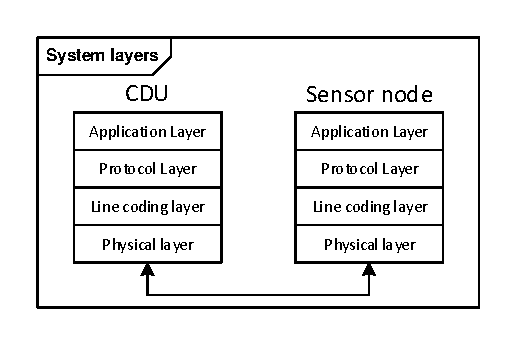
\includegraphics[width=.6\textwidth]{billeder/11ProjectDescription/System_Layers}
	\caption{System Layers}
	\label{fig:systemlayers}
\end{figure}
Conceptual designs of the different parts of the system are made by taking the blocks from the system overview (figure \ref{fig:systembdd}) and creating internal block diagrams.\\
The CDU is comprised of six conceptual blocks as seen on figure \ref{CDU_IBD}. Each block has a unique responsibility. For instance the sensor power supply has the responsibility of powering the sensors. The sensor power supply block and sensor communication block makes up the physical layer with regards to figure \ref{fig:systemlayers} while the line coding and protocol layer is handled by the µ-Controller block. 
\begin{figure}[hbpt]
	\centering
	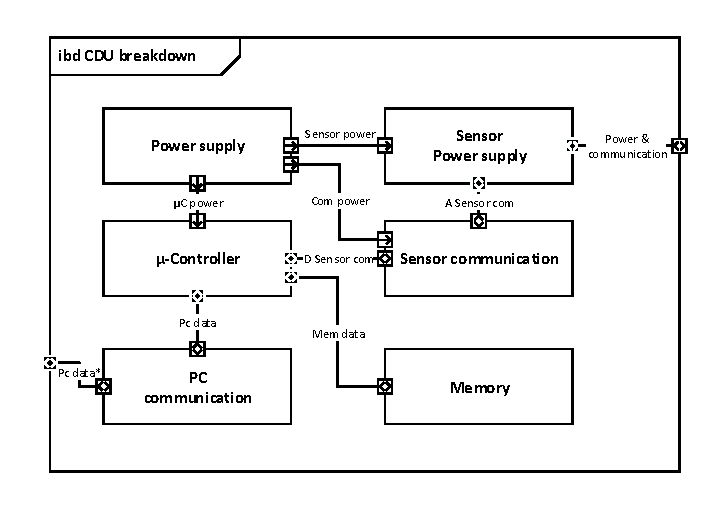
\includegraphics[width=.8\textwidth]{billeder/11ProjectDescription/CDU_IBD}
	\caption{Internal Block Diagram of the CDU}
	\label{CDU_IBD}
\end{figure}
A sensor node can be divided into 4 conceptual blocks as seen on figure \ref{fig:SN_IBD}. The Power supply block and the Communication block make up the physical layer as described in the CDU. The line coding and protocol layer is handled by the Logic handler block.
\begin{figure}[hbpt]
\centering
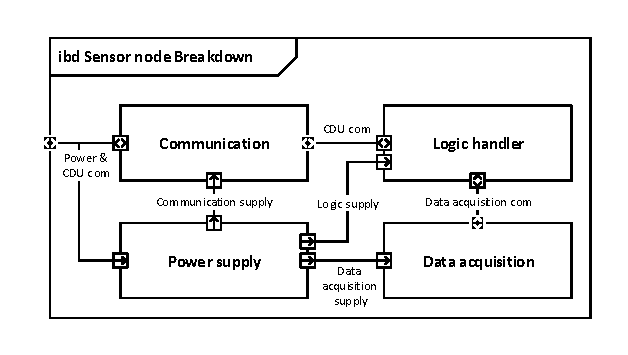
\includegraphics[width=.8\textwidth]{billeder/11ProjectDescription/Sensor_IBD}
\caption{Internal Block Diagram of the sensor node}
\label{fig:SN_IBD}
\end{figure}

Communication on the bus can be broken down to a series of steps. The CDU takes the initiative to write to a sensor node. It creates the message that will be sent and starts transmitting. The message is received on the sensor node and the sensor node starts processing the message. When it is finished processing it will respond according to the message. The response is received on the CDU where it will be processed. This transmission sequence can be seen on figure \ref{fig:sintrans}. The figure also shows the flow of information through the layers. 
\begin{figure}[hbpt]
\centering
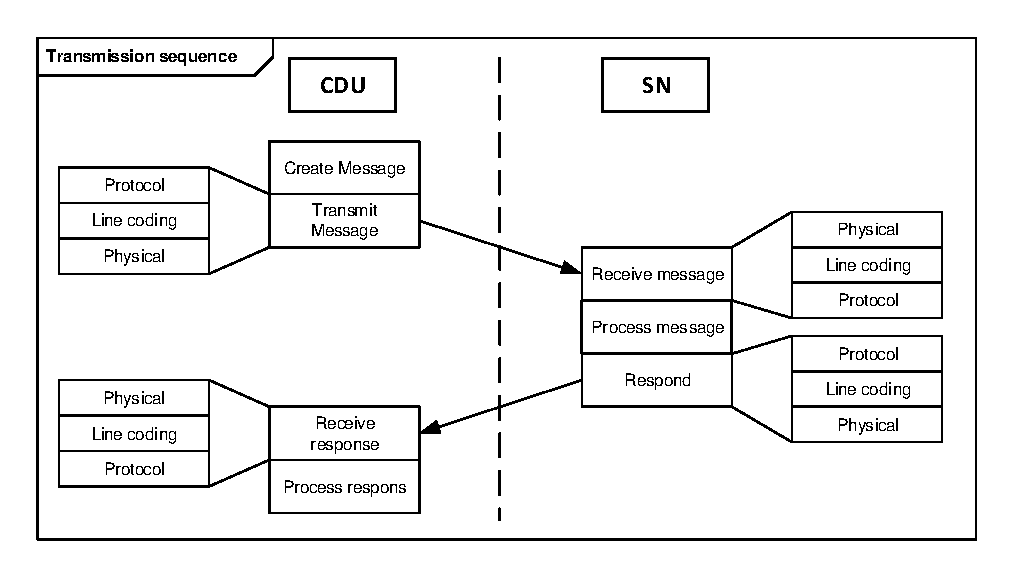
\includegraphics[width=.8\textwidth]{billeder/11ProjectDescription/singletransmission}
\caption{A single transmission}
\label{fig:sintrans}
\end{figure}

The protocol layer (or protocol) was designed with the knowledge from the technology study. A full header can be seen in table \ref{table:stdmsgtosensor}. The DLM(Data Length Multiplier) determines how many bytes of data will be sent up to a maximum of 15 bytes. If there is no data the DLM is zero.
\begin{table}[hbpt]
\centering
\begin{tabular}{|l|l|l|l|l|l|}
	\hline
	Start Sequence & Address & Function Code & DLM & Data & CRC  \\ \hline
	1 nibble & 1 nibble	& 1 nibble & 1 nibble & n bytes & 1 byte\\
	\hline
\end{tabular}
\caption{Message format for writing and reading}
\label{table:stdmsgtosensor}
\end{table}
The CRC check ensures that the message has been received correctly.

\section{Design and implementation}
The design and implementation of the system is a naturally continuation of the technology study made in this project. The key part was integrating the acquired knowledge from the study and applying it to design and implement the prototype system.\\
When taking the system layers into consideration (figure \ref{fig:systemlayers}), the protocol and line coding layers fits well into software design. The physical layer matches hardware design and implementation.\\
The design of the physical hardware layer was derived from the technology study of how a communication bus could be made. The central parts of the communication is carrying the communication and the conversion from digital levels to something that can be carried by the bus.\\ 
The technology study led to a current loop being used to communicate with the sensor nodes. Two different current levels corresponds to logic 0(low) and 1(high). When responding, the sensor nodes use two different voltage levels.\\
The conversion from digital levels to analog current levels is handled by two block in the CDU: The Sensor power supply block (figure \ref{fig:CDUSPS}) and the Sensor communication block (figure \ref{fig:CDUSC}).\\
\begin{figure}[H]
	\begin{minipage}[b]{0.45\linewidth}
	\centering
	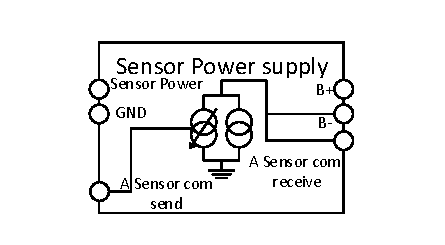
\includegraphics[scale=1]{billeder/11ProjectDescription/CDUSPS}
	\caption{Detailed CDU Sensor Power supply design.}
	\label{fig:CDUSPS}
	\end{minipage}
	\hspace{0.5cm}
	\begin{minipage}[b]{0.45\linewidth}
	\centering
	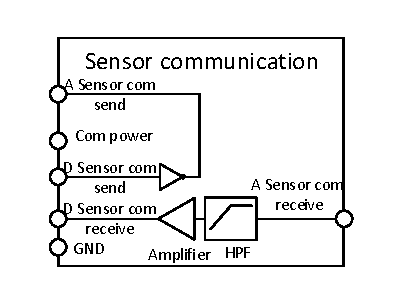
\includegraphics[scale=1]{billeder/11ProjectDescription/CDUSC}
	\caption{Detailed CDU Sensor communication design.}
	\label{fig:CDUSC}
	\end{minipage}
\end{figure}
Each sensor node will react to the difference in current levels. The current is converted to a voltage in the power supply block of the sensor node (figure \ref{fig:SN_PS_FIGURE}). The voltage levels are then converted to digital levels by the communication block of the sensor node(figure \ref{fig:SN_com_fig}). The digital levels are handled by the logic handler which will be described later in this chapter.\\
\begin{figure}[H]
	\begin{minipage}[b]{0.45\linewidth}
	\centering
	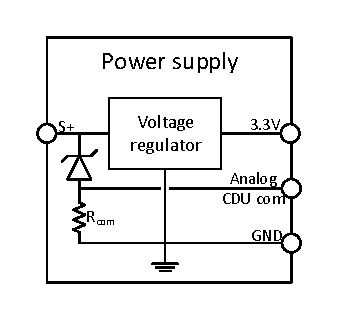
\includegraphics[width=0.8\textwidth]{billeder/11ProjectDescription/powersupply_detailed_sn}
	\caption{Sensor node power supply block}
	\label{fig:SN_PS_FIGURE}
	\end{minipage}
	\begin{minipage}[b]{0.45\linewidth}
	\centering
	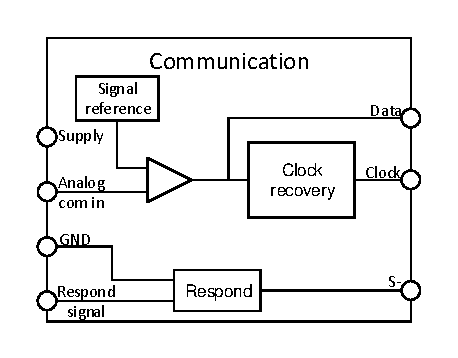
\includegraphics[width=1\textwidth]{billeder/11ProjectDescription/communication_sn}
	\caption{Sensor node communication block}
	\label{fig:SN_com_fig}
	\end{minipage}
\end{figure} 
Responding starts once the addressed sensor node has finished chewing through the message it has received. The digital level signal is converted to two different voltage levels by the communication block of the sensor node. The voltage levels on the bus is then directed from the sensor power supply of the CDU to the sensor communication block of CDU. The voltage levels will then be converted to digital logic levels and handled by the CDU.

\section{Tests}
\textit{The tests section seeks to explain the methods, reasons and procedures for testing in this project.}\\

The internal tests in this project is made up of unit tests and integration tests. The unit tests seek to tests the functionality of each device while the integration tests are designed to tests the communication in between devices.\\

The unit tests were made such that there were as few variable circumstances as possible. This means possible errors will most certainly stem from the unit under test (uut). This principle of testing was also applied when unit testing.\\

The tests made in this project are by no means exhaustive. The tests made are suppose to provide a baseline for improving the system or otherwise prove a basic concept. As the outcome of this project is a technology and not an actual product there is no accept-test.\\

The full extent of tests are:\\
Integration:\\
\begin{itemize}
\item Integration test case 1: Sensor getinfo request
\item Integration test case 2: Sensor getdata request
\item Integration test case 3: Sensor respond to getinfo
\item Integration test case 4: Sensor respond to getdata
\item Integration test case 5: Full transmission
\item Integration test case 6: Full transmission, unknown function code
\item Integration test case 7: PC sends getdata request to CDU
\item Integration test case 8: PC sends unknown request to CDU
\end{itemize}
Reliability:\\
\begin{itemize}
\item Reliability test case 1: Timed transmissions and errors
\end{itemize}
CDU unit tests:\\
\begin{itemize}
\item Test case 1: 3.3 volt power supply
\item Test case 2: Communcation to bus
\item Test case 3: Voltage reference in receiver circuit
\item Test case 4: Communication from bus
\item Test case 5: Test of function IntegerToBinary
\item Test case 6: Test of function PatMessage
\item Test case 7: Test of function ToManchester
\item Test case 8: Test of function InitSensorArray
\item Test case 9: Test of function CDUSend
\item Test case 10: Test of function CDUReceive
\item Test case 11: Test of function CDUReceive error handling
\end{itemize}
Sensor node unit tests:\\
\begin{itemize}
\item Test case 1: 3.3 volt power supply
\item Test case 2: Data recovery circuit
\item Test case 3: Phase lock circuit
\item Test case 4: Respond circuit
\item Test case 5: CDU communication
\item Test case 6: ADC interfacing
\end{itemize}
The content of a test can be explained on the basis of integration test case 1 which can be found in the Internal tests document in the appendixa. Each test case contains the purpose of the tests, which tests equipment is used in the test, the procedure, the expected result and the actual result.\\ 
The purpose explains what is being tested. The test equipment used includes stubs of the units that are being tested. This could be a sensor stub needed for testing the CDU or a full sensor node tests stub used for testing communication. The procedure seeks to explain how to do the tests in a way such that a technician can perform the test without prior knowledge to the system. The expected result provides a range or a basis on which the actual result can be evaluated.\\